\documentclass{article}

\usepackage{fancyhdr} % Required for custom headers
\usepackage{lastpage} % Required to determine the last page for the footer
\usepackage{extramarks} % Required for headers and footers
\usepackage[usenames,dvipsnames]{color} % Required for custom colors
\usepackage{graphicx} % Required to insert images
\usepackage{listings} % Required for insertion of code
\usepackage{courier} % Required for the courier font
\usepackage{booktabs} % Used for inserting dummy 'Lorem ipsum' text into the template
\usepackage{fancyvrb}

% Margins
\topmargin=-0.45in
\evensidemargin=0in
\oddsidemargin=0in
\textwidth=6.5in
\textheight=9.0in
\headsep=0.25in

\linespread{1.1} % Line spacing

% Set up the header and footer
\pagestyle{fancy}
\lhead{\tutorialAuthorName} % Top left header
\chead{\hmwkTitle} % Top center head
\rhead{}%\firstxmark} % Top right header
\lfoot{\lastxmark} % Bottom left footer
\cfoot{} % Bottom center footer
\rfoot{Page\ \thepage\ of\ \protect\pageref{LastPage}} % Bottom right footer
\renewcommand\headrulewidth{0.4pt} % Size of the header rule
\renewcommand\footrulewidth{0.4pt} % Size of the footer rule

\setlength\parindent{0pt} % Removes all indentation from paragraphs

%----------------------------------------------------------------------------------------
% CODE INCLUSION CONFIGURATION
%----------------------------------------------------------------------------------------

\definecolor{MyDarkGreen}{rgb}{0.0,0.4,0.0} % This is the color used for comments
\lstloadlanguages{Java} % Load Perl syntax for listings, for a list of other languages supported see: ftp://ftp.tex.ac.uk/tex-archive/macros/latex/contrib/listings/listings.pdf
\lstset{language=Java, % Use Perl in this example
        frame=single, % Single frame around code
        basicstyle=\small\ttfamily, % Use small true type font
        keywordstyle=[1]\color{Blue}\bf, % Perl functions bold and blue
        keywordstyle=[2]\color{Purple}, % Perl function arguments purple
        keywordstyle=[3]\color{Blue}\underbar, % Custom functions underlined and blue
        identifierstyle=, % Nothing special about identifiers
        commentstyle=\usefont{T1}{pcr}{m}{sl}\color{MyDarkGreen}\small, % Comments small dark green courier font
        stringstyle=\color{Purple}, % Strings are purple
        showstringspaces=false, % Don't put marks in string spaces
        tabsize=5, % 5 spaces per tab
        %
        % Put standard Perl functions not included in the default language here
        morekeywords={rand},
        %
        % Put Perl function parameters here
        morekeywords=[2]{on, off, interp},
        %
        % Put user defined functions here
        morekeywords=[3]{test},
        %
        morecomment=[l][\color{Blue}]{...}, % Line continuation (...) like blue comment
        numbers=left, % Line numbers on left
        firstnumber=1, % Line numbers start with line 1
        numberstyle=\tiny\color{Blue}, % Line numbers are blue and small
        stepnumber=5 % Line numbers go in steps of 5
}

% Creates a new command to include a perl script, the first parameter is the filename of the script (without .pl), the second parameter is the caption
\newcommand{\perlscript}[2]{
\begin{itemize}
\item[]\lstinputlisting[caption=#2,label=#1]{#1.pl}
\end{itemize}
}

%----------------------------------------------------------------------------------------
% DOCUMENT STRUCTURE COMMANDS
% Skip this unless you know what you're doing
%----------------------------------------------------------------------------------------

% Header and footer for when a page split occurs within a problem environment
\newcommand{\enterProblemHeader}[1]{
\nobreak\extramarks{#1}{#1}\nobreak
\nobreak\extramarks{#1 (continued)}{#1 }\nobreak
}

% Header and footer for when a page split occurs between problem environments
\newcommand{\exitProblemHeader}[1]{
\nobreak\extramarks{#1 (continued)}{#1 continued on next page\ldots}\nobreak
\nobreak\extramarks{#1}{}\nobreak
}

\setcounter{secnumdepth}{0} % Removes default section numbers
\newcounter{homeworkProblemCounter} % Creates a counter to keep track of the number of problems

\newcommand{\homeworkProblemName}{}
\newenvironment{homeworkProblem}[1][Section \arabic{homeworkProblemCounter}]{ % Makes a new environment called homeworkProblem which takes 1 argument (custom name) but the default is "Problem #"
\stepcounter{homeworkProblemCounter} % Increase counter for number of problems
\renewcommand{\homeworkProblemName}{#1} % Assign \homeworkProblemName the name of the problem
\section{\homeworkProblemName} % Make a section in the document with the custom problem count
\enterProblemHeader{\homeworkProblemName} % Header and footer within the environment
 }{
\exitProblemHeader{\homeworkProblemName} % Header and footer after the environment
}

\newcommand{\problemAnswer}[1]{ % Defines the problem answer command with the content as the only argument
\noindent\framebox[\columnwidth][c]{\begin{minipage}{0.98\columnwidth}#1\end{minipage}} % Makes the box around the problem answer and puts the content inside
}

\newcommand{\homeworkSectionName}{}
\newenvironment{homeworkSection}[1]{ % New environment for sections within homework problems, takes 1 argument - the name of the section
\renewcommand{\homeworkSectionName}{#1} % Assign \homeworkSectionName to the name of the section from the environment argument
\subsection{\homeworkSectionName} % Make a subsection with the custom name of the subsection
\enterProblemHeader{\homeworkProblemName\ }% [\homeworkSectionName]} % Header and footer within the environment
}{
\enterProblemHeader{\homeworkProblemName} % Header and footer after the environment
}

%----------------------------------------------------------------------------------------
% NAME AND CLASS SECTION
%----------------------------------------------------------------------------------------

\newcommand{\hmwkTitle}{Jannovar Tutorial} % Assignment title
\newcommand{\version}{January 18,\ 2014} % Due date
\newcommand{\tutorialAuthorName}{Peter Robinson} % Your name

%----------------------------------------------------------------------------------------
% TITLE PAGE
%----------------------------------------------------------------------------------------

\title{
\vspace{2in}
\textmd{\textbf{\sc Jannovar Tutorial}}\\
\normalsize\vspace{0.1in}\small{Version\ of\ \version}\\
\vspace{3in}
}

\author{\textbf{\tutorialAuthorName}}
\date{} % Insert date here if you want it to appear below your name

%----------------------------------------------------------------------------------------

\begin{document}

\maketitle

%----------------------------------------------------------------------------------------
% TABLE OF CONTENTS
%----------------------------------------------------------------------------------------

%\setcounter{tocdepth}{1} % Uncomment this line if you don't want subsections listed in the ToC

\newpage
\tableofcontents
\newpage

%----------------------------------------------------------------------------------------
% PROBLEM 1
%----------------------------------------------------------------------------------------

% To have just one problem per page, simply put a \clearpage after each problem

\begin{homeworkProblem}[1. Getting Started with Jannovar]

Jannovar is a stand-alone Java program for annotating VCF files from whole-exome sequencing. Thus, Jannovar translates the information from the VCF file on the chromosomal location of variants into gene- and transcript-based annotations. Jannovar is also a Java library that can be used to develop sophisticated new Java applications  for exome analysis (and similar applications). In addition to its functionality in annotating variants, Jannovar can also perform simple pedigree analysis of the kind that is becoming common in exome sequencing projects in human genetics.

The basic problem that Jannovar is designed to solve is the fact that variant calling programs report variants using chromosomal coordinates, but medical or biological interpretation of the data almost always requires the prediction of the 
effects of the variants on individual transcripts. Therefore, an annotation program must interpret chromosomal variants by determining what gene and transcripts are affected by the variants and how. For instance, if we find the variant \verb+chr17:g.18647625T>A+, we would like to know that it affects the \textit{FBXW10} gene, that four different transcripts of that gene are affected, including \verb+uc002guj.3+. The variant affects exon 1 of that transcript, causing a T to A transversion (\verb+c.68T>A+), predicted to lead to the substitution of an isoleucine by an asparagine residue (\verb+p.I23N+).


This document first explains how to use the standalone program and then gives some examples of how to use the  
Jannovar library for programming.

\end{homeworkProblem}

\begin{homeworkProblem}[2. Downloading Jannovar]

Most users will want to download the main Jannovar file from the project homepage at 
compbio.charite.de.\footnote{Complete URL: http://compbio.charite.de/contao/index.php/jannovar.html} To perform the following exercises, you will need only the file \texttt{Jannovar.jar}. 

Alternatively, the complete source code can be downloaded as a maven repository with additional junit code for unit testing from GitHub at \texttt{https://github.com/charite/jannovar}. To perform the following steps, you will need to have git and maven installed on your computer.

To download the repository, enter:

\begin{verbatim}
$ git clone https://github.com/charite/jannovar
\end{verbatim}

To build the package, enter

\begin{verbatim}
$ cd jannovar
$ mvn package
\end{verbatim}

This will create the file \texttt{Jannovar.jar}. Note that maven will first conduct some unit tests (tests to check that the software is working correctly) before it creates the executable file, which will be located in the subdirectory ``\texttt{target}''.
\end{homeworkProblem}


%%%%%%%%%%%%%%%%%%%%%%%%%%%%%%%%%%%%%%%%%%%%%%%%%%%%%%%%%%%%%%%%%%%%%%%%%%%
%%%%%%%%%%%%%%%%%%%%%%%%%%%%%%%%%%%%%%%%%%%%%%%%%%%%%%%%%%%%%%%%%%%%%%%%%%%



\begin{homeworkProblem}[3. Reserving Memory for Jannovar]
Java programs are be compiled into Java bytecode, a standardized portable binary format which in theory can be compiled once and then run on any platform (this led to Sun's slogan, ``Write once, run anywhere''). Java programs may consist either of a number of class files or for easier distribution, the class files may be packaged together in a .jar file (short for Java archive, this is how things are done with Jannovar). Java programs then run on a Java Virtual Machine (JVM) which verifies and executes the bytecode.

The JVM runs with fixed available memory. Once this memory is exceeded, a \texttt{java.lang.OutOfMemoryError} will occur. The JVM tries to make an intelligent choice about the available memory at startup, but if the program runs out of memory, it will crash (this is different from C programs, that may be able to obtain more memory from the operating system). 

There are two important settings to adjust the amount of memory used by the JVM.

\begin{center}
\begin{tabular}{ll}
 -Xms1g & Set the minimum available memory for the JVM to 1 Gigabyte\\
-Xmx2g & Set the maximum available memory for the JVM to 2 Gigabyte.\\
\end{tabular}
\end{center}

These parameters can be set from the command line or as system-wide settings. On Windows, for instance, one would go to the 
 Control Panel,  click on \texttt{Programs}, g to Java settings, click on "Java Control Panel", and then go to "Runtime Parameters" and change the value, or if it is blank decide for the new value, of the Java memory (the two parameters shown above). 

On Linux systems, this can be done by adding the following line to your Bash profile

\begin{verbatim}
JAVA_TOOL_OPTIONS="-Xms2G -Xmx2G"
\end{verbatim}

It may be preferable just to pass these arguments on the command line as follows (here we have reserved a minimum and maximum of 2 Gigabytes memory for the JVM):

\begin{verbatim}
$ java -Xms2G -Xmx2G -jar Jannovar.jar [options]
\end{verbatim}
\end{homeworkProblem}

%%%%%%%%%%%%%%%%%%%%%%%%%%%%%%%%%%%%%%%%%%%%%%%%%%%%%%%%%%%%%%%%%%%%%%%%%%%
%%%%%%%%%%%%%%%%%%%%%%%%%%%%%%%%%%%%%%%%%%%%%%%%%%%%%%%%%%%%%%%%%%%%%%%%%%%
\begin{homeworkProblem}[4. Understanding and Creating the Transcript Definition File]

Jannovar is designed to use transcript data from the UCSC Genome Browser database (known genes), ensembl, or NCBI refseq.  
The data comprises information about the chromosomal locations of transcripts, their exons, strands, the corresponding mRNA sequences, and several cross-references to other databases. 

The the UCSC known genes data, Jannovar uses four different files from the UCSC data base (note that by default, the hg19 versions are used):
\begin{itemize}
 \item knownGene.txt
 \item knownGeneMrna.txt
\item kgXref.txt
\item knownToLocusLink.txt
\end{itemize}

Jannovar will automatically download these files from the UCSC FTP site. To do this, enter 

 \begin{verbatim}
$ java -jar Jannovar.jar --create-ucsc 
 \end{verbatim}

 



This will cause Jannovar to create a directory called \texttt{data} with subdirectory \texttt{hg19},  to download the four files into it (note: the files are compressed in gzip format and do not need to be uncompressed), and then it will create a file called \textbf{ucsc\_hg19.ser} in the \texttt{data} directory. This is a so-called serialized file,\footnote{A serialized object is a software object (in our case, a list of objects representing the approximately 70,000 transcript models) that has been converted into a byte stream and written to a file. This file can now easily be read and quickly converted back to the original software objects, simplifying and accelerated the analysis.} meaning essentially that the data that is needed for the computational analysis is stored in a form that allows easy and quick input from a single file, rather than requiring the original files to be reparsed every time we do the analysis.

Analogously, to download data and create a transcript definition file for Ensembl transcripts, enter

\begin{verbatim}
$ java -jar Jannovar.jar --create-ensembl 
\end{verbatim}
Finally, to create a transcript definition file for NCBI RefSeq transcripts, enter
\begin{verbatim}
$ java -jar Jannovar.jar --create-refseq 
\end{verbatim}

\begin{homeworkSection}{Other genome builds}
You can also use the -g option followed by one of mm9, mm10, hg18, hg19 to
download the data from the mouse genome (builds mm9 or mm10) as well as data from the previous human genome build hg18. This will create new subdirectories in the data directory corresponding to the build name.
\end{homeworkSection}

\begin{homeworkSection}{Setting the proxy}
If you live behind a firewall, you may need to set the proxy and the proxy port accordingly. This is done with the --proxy and the --proxy-port flags.
\begin{verbatim}
$ java -jar Jannovar.jar --create-ucsc \
        --proxy proxy.example.edu --proxy-port 123
 \end{verbatim}
\end{homeworkSection}

\begin{homeworkSection}{Using local files}
If the four UCSC files have been previously downloaded and are located (compressed or uncompressed) in the directory \texttt{data/hg19}, then one can also serialize them with the following command.
\begin{verbatim}
$ java -jar Jannovar.jar -S data/hg19
\end{verbatim}
\end{homeworkSection}

\end{homeworkProblem}
%%%%%%%%%%%%%%%%%%%%%%%%%%%%%%%%%%%%%%%%%%%%%%%%%%%%%%%%%%%%%%%%%%%%%%%%%%%
%%%%%%%%%%%%%%%%%%%%%%%%%%%%%%%%%%%%%%%%%%%%%%%%%%%%%%%%%%%%%%%%%%%%%%%%%%%
\begin{homeworkProblem}[5. Annotating VCF files]

Jannovar can now be used to annotate a VCF file (with a single sample or with multiple samples). Of course, the variant calls in the VCF file needs to have be done using  coordinates that match those of the transcript definition file (e.g., both the VCF file and the transcript definition file need to be hg19). 

In this mode, Jannovar will add the variant type and a representative annotation to each line of the VCF file. It will write the annotated VCF to a new file with the same name as the original file but with a the suffix ``jv.vcf'' instead of ``vcf''. 

\begin{verbatim}
$ java -jar Jannovar.jar -D ucsc_hg19.ser -V example.vcf
\end{verbatim}

This command uses the \texttt{ucsc\_hg19.ser} file created as above (use the -D flag followed by the path if the \texttt{ucsc.ser} file is in another directory). The -V flag indicates the path to a VCF file to be annotated. This command will create a new file called \verb+example.jv.vcf+. For instance, if the original VCF file has the line

\begin{verbatim}
1	155981489	rs1475766	C	G	190.78	PASS	AC=1;AF=0.50;AN=2;...
\end{verbatim}

then Jannovar will append a representative functional annotation to the beginning of the INFO field (i.e., the field that starts with \verb+AC=1;AF=0.50;AN=2;...+):

\begin{verbatim}
EFFECT=UTR3;HGVS=SSR2:uc010pgw.2:c.*3242G>C;AC=1;AF=0.50;AN=2;...
\end{verbatim}

That is, the EFFECT field indicates the class of variant, and the HGVS field shows a representative annotation for the variant (note that variants often affect multiple transcripts; we will see in the next section how to use Jannovar to see all possible transcripts).	This can be useful both for human inspection as well as for software pipelines that use VCF files for their analysis, since this format makes it easy to parse out the variant class, the affect gene, and a representative annotation. The annotations are listed according to their priority. That is, if the same variant leads to a NONSENSE mutation in a coding transcript, and also affects a noncoding transcript, Jannovar will show the NONSENSE variant in this place. Table~\ref{tab:priority} shows the priority levels of different classes of variant.



\begin{table}[!ht]
\begin{center}
\begin{tabular}{llp{10cm}}
\toprule
Symbol & Pr. & Example \\
\midrule
MISSENSE & 1 & \verb+GMPR:NM_006877.3:exon8:c.766T>A:p.F256I+
\\
FS\_DELETION & 1 & \verb+ZNF675:NM_138330.2:exon3:c.204delT:p.H68fs+\\
FS\_INSERTION  & 1 &  \verb+FBN1:NM_000138.4:exon9:c.864_865insC:p.I289fs+ \\
FS\_SUBSTITUTION  & 1 & \verb+OR51I2:NM_001004754.2:exon1:c.713_714delinsGTGT:p.L238fs+
 \\
NON\_FS\_DELETION & 1 &  \verb+MESP2:NM_001039958.1:exon1:c.545_547del:p.Q182_G183delR+ \\
NON\_FS\_INSERTION  & 1 &  \verb+CDK11A:XM_005244784.1:exon5:c.350_351insTCC:p.R117delinsSP+\\
NON\_FS\_SUBSTITUTION  & 1 & \verb+MESP2:NM_001039958.1:exon1:c.544_552delinsTTT:+\newline \verb+p.Q182_Q184delinsF+ \\
SPLICING & 1& \verb!NIPAL2:NM_024759.1:exon11:c.1067+1G>A!\\
STOPGAIN  & 1 &  \verb+OR1B1:NM_001004450.1:exon1:c.574C>T:p.R192*+ \\
STOPLOSS  & 1 &  \verb+CENPN:NM_018455.5:exon7:c.613T>G:p.*205E+ \\
FS\_DUPLICATION & 1 & \verb+DGKK:NM_001013742.2:exon22:c.3061dupC:p.L1021fs+\\
NON\_FS\_DUPLICATION&1& \verb+C8orf59:NM_001099673.1:exon4:c.265_270dupAATGTT:p.N89_V90dup+\\
STARTLOSS & 1 & \verb+KRTAP4-8:NM_031960.2:exon1:c.1_2insC:p.M1?+\\
\midrule
ncRNA\_EXONIC  & 2 &  \verb+PLEKHH3:NR_073574.1:exon4:n.1306G>A+ \\
ncRNA\_SPLICING  & 2 & \verb!TBC1D3P5:uc002gzg.3:exon11:n.1595+2C>T! \\
\midrule
UTR3 & 3 & \verb+G6PC:NM_000151.3:c.*23T>C+ \\
\midrule
UTR5 & 4 &  \verb+HEXIM1:NM_006460.2:c.-80C>T+\\
\midrule
SYNONYMOUS & 5&  \verb+PLEKHM1:NM_014798.2:exon4:c.852C>T:p.C284C+ \\
\midrule
INTRONIC & 6 &  \verb!ITGB3:NM_000212.2:intron11:c.1914-19T>C! \\
\midrule
ncRNA\_INTRONIC & 7 &  \verb!MRPL10:NR_037575.1:intron3:n.567-16T>C! \\
\midrule
UPSTREAM & 8 & NDUFA7(dist=87) \\
DOWNSTREAM & 8 & GNRH2(dist=24) \\
\midrule
INTERGENIC & 9 &  ENTPD4(dist=25494):SLC25A37(dist=45625) \\
\midrule
ERROR & 10 & - \\
\bottomrule
\end{tabular}
\end{center}

\caption{The variant classes recognized by Jannovar. FS stands for frameshift, thus 
NON\_FS\_INSERTION refers to a non-frameshift insertion etc. Every variant in a valid VCF file should
correspond to one of these classes. \textit{Pr}. stands for the Priority level of the given variant class.
Note that we show annotations to NCBI RefSeqs in this table, but we use UCSC identifiers in the remainder of this tutorial.}
\label{tab:priority}
\end{table}

\end{homeworkProblem}
%%%%%%%%%%%%%%%%%%%%%%%%%%%%%%%%%%%%%%%%%%%%%%%%%%%%%%%%%%%%%%%%%%%%%%%%%%%
%%%%%%%%%%%%%%%%%%%%%%%%%%%%%%%%%%%%%%%%%%%%%%%%%%%%%%%%%%%%%%%%%%%%%%%%%%%

\begin{homeworkProblem}[6. Creating Separate, Comprehensive Annotation Files]

Sometimes it is desirable to know all of the potential annotations associated with some variant. While the VCF annotation functionality produces one representative annotation, it is also possible to generate a separate file with a comprehensive annotation list (one for each affected transcript). To do so, just add a -J flag to the above command. 


\begin{verbatim}
$ java -jar Jannovar.jar -D ucsc_hg19.ser -V example.vcf -J
\end{verbatim}
This command uses the \texttt{ucsc\_hg19.ser} file created as above (use the -D flag followed by the path if the \texttt{ucsc\_hg19.ser} file is in another directory). The -V flag indicates the path to a VCF file to be annotated. 
The -J flag indicates that Jannovar should create a Jannovar-format output file with a comprehensive list of annotations. 
This command will create a new file called \verb+example.vcf.jannovar+. For instance, the following shows annotations for a variant at position 44112873 of chromosome 7 that affects four different transcripts of the \textit{POLM} gene.
\begin{small}

\begin{verbatim}
14359	Nonsynonymous	POLM	uc003tjx.2:exon9:c.1315C>A:p.H439N	chr7	44112873	G	T	0/1	260.0
14359	ncRNA_exonic	POLM	uc003tjv.3:exon1:n.1565C>A	chr7	44112873	G	T	0/1	260.0
14359	UTR3	POLM	uc003tju.3:c.*17C>A	chr7	44112873	G	T	0/1	260.0
14359	UTR3	POLM	uc003tjt.3:c.*17C>A	chr7	44112873	G	T	0/1	260.0
\end{verbatim}              \end{small}


\end{homeworkProblem}
%%%%%%%%%%%%%%%%%%%%%%%%%%%%%%%%%%%%%%%%%%%%%%%%%%%%%%%%%%%%%%%%%%%%%%%%%%%
%%%%%%%%%%%%%%%%%%%%%%%%%%%%%%%%%%%%%%%%%%%%%%%%%%%%%%%%%%%%%%%%%%%%%%%%%%%

\begin{homeworkProblem}[7. Writing Java Code with the Jannovar Library]
 
We have used the Jannovar code basis as a Java library that now is part of the Exomiser project.\footnote{\begin{scriptsize}http://www.sanger.ac.uk/resources/databases/exomiser/                                                                                                                                                               \end{scriptsize}} Our goal was to make a modular, well tested, and easily extensible software library that could be used by us and others for larger software projects. This document explains the application programming interface (API) or Jannovar and provides several examples of how one might use Jannovar as a component of applications that perform filtering or analysis of whole exome sequence (WES) data using user-defined algorithms. Jannovar provides easy to use annotation of the VCF data as well as the capability of combining VCF analysis with simple pedigree analysis if pedigree data in the form of a PED file is provided.

The file \texttt{Jannovar.java}, which is part of the Jannovar distribution (see
Section~2), provides a complete example of how to annotate VCF Files (see especially \texttt{outputAnnotatedVCF} and \texttt{annotateVCFLine} or to output annotations in a user-defined format (see especially the methods \texttt{outputJannovarFormatFile} and \texttt{outputJannovarLine}). The code in \texttt{Jannovar.java} is extensively documented and provides an easy starting point to develop sophisticated analysis pipelines for exome sequencing. In the next section, we will explain a complete but simple example that demonstrates many of the features of the Jannovar library but avoids bells and whistles. The demo program will show how to use Jannovar to filter VCF files according to pedigree analysis and then output a list of genes and variants that correspond to a give pattern of inheritance. But before we explain that code, we will review the PED file format that is used by Jannovar to represent pedigree information.
 
\begin{homeworkSection}{Comment: Why not add pedigree filtering to the Jannovar executable?}
 In general, family-based filtering of exome data searches for candidate mutations that are distributed in a pedigree as one would expect for a given mode of inheritance. For instance, in the case of an autosomal dominant disease, one searches for potentially pathogenic variants that are heterozygous in all affected individuals and not present in all unaffected individuals. Since Jannovar does not filter out common variants, there would be a high number of false positive hits if Jannovar were the only tool used to perform pedigree analysis. Instead, it makes more sense to use this feature of Jannovar as a component in an analysis program that filters variants according to user-defined criteria. 
\end{homeworkSection}


\end{homeworkProblem}

%%%%%%%%%%%%%%%%%%%%%%%%%%%%%%%%%%%%%%%%%%%%%%%%%%%%%%%%%%%%%%%%%%%%%%%%%%%
%%%%%%%%%%%%%%%%%%%%%%%%%%%%%%%%%%%%%%%%%%%%%%%%%%%%%%%%%%%%%%%%%%%%%%%%%%% 


\begin{homeworkProblem}[7. Understanding PED files]
The Jannovar code base provides functionality for integrating simple pedigree analysis into exome analysis pipelines. Before we explain how to use this feature, we offer a brief explanation of the PED file format that can be skipped by readers familiar with it.





A PED file ('Pedigree file') describes the family relationships of each sample 
along with their gender and phenotype. PED files are typically used by software that
performs genetic linkage analysis. Jannovar can perform simple pedigree analysis based on 
 a PED file corresponding to a VCF file that contains samples from all of the persons mentioned in the PED file. 

\begin{homeworkSection}{The PED file}

The PED file is white-space (space or tab) delimited and should have no header and exactly six columns. 

\begin{center}
\begin{tabular}{lllp{7cm}}
\toprule
Column & Item & Example & Explanation\\
\midrule
1 & Family ID & FAM001 & An identifier for the family.\\
2 & Sample ID & \verb+859_A+ & A unique identifier for the sample (person). \\
3 & Father's sample ID & \verb+922_B+ & The sample ID for the father of the current individual (or 0 if the father is not represented in the pedigree)\\
4 & Mother's sample ID & \verb+923_B+ & The sample ID for the mother of the current individual (or 0 if the mother is not represented in the pedigree)\\
5 & Gender & 2 & 1 for male, 2 for female, 0 if unknown. \\
6 & Phenotype & 1 & 1 for unaffected, 2 for affected, 0 if unknown. \\
\bottomrule
\end{tabular}
\end{center}

\end{homeworkSection}

\begin{homeworkSection}{Autosomal recessive pedigrees}

Figure~\ref{fig:ar} shows a family that is segregating a disease with autosomal recessive inheritance.


\begin{figure}[!ht]
 \centering
 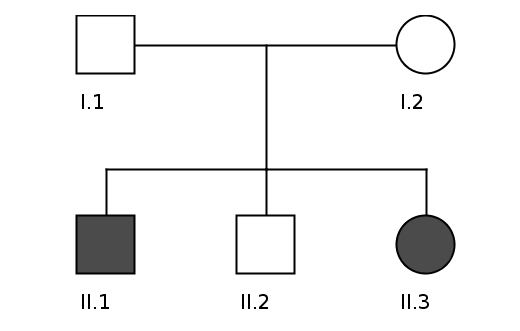
\includegraphics[width=.4\textwidth]{./img/ARpedigree.png}
\caption{An example pedigree representing a family segregating an autosomal recessively inherited disease. The parents are assumed to be heterozygous mutation carriers. In this case, each affected child can either homozygous for a mutation in the disease gene, and both parents are heterozygous carriers, or alternatively the children are all compound heterozygous for two distinct mutations in the same gene, and the parents are heterozygous carriers of one mutation each -- different in each parent. Here, the son II.1 is affected, the son II.2 is healthy (and thus can be heterozygous for maximally one mutation), and the daughter II.3 is affected.}
\label{fig:ar}
\end{figure}

\vspace{2cm}
For the family shown in Figure~\ref{fig:ar}, we can write the PED file as follows:

\begin{Verbatim}[frame=single]
FAM1	I.1	 0	  0	  1	1
FAM1	I.2	 0	  0	  2	1
FAM1	II.1	I.1	I.2	1	2
FAM1	II.2	I.1	I.2	1	1
FAM1	II.3	I.1	I.2	2	2
\end{Verbatim}

Note that we can use an arbitrary family ID in the first column. Jannovar is designed to analyze only single families and will report an error if it is attempted to analyze a PED file with multiple families. For autosomal recessive pedigrees, only one set of parents is allowed (that is, analysis is restricted to a nuclear family).

\end{homeworkSection}
\begin{homeworkSection}{Homozygous and compound heterozygous variants}
In some situations it may be desirable to screen for homozygous or  compound heterozygous variants that are
compatible with autosomal recessive inheritance. For instance, in consanguineous families, homozygous (i.e., autozygous) mutations are commonly found, whereas in outbred families segregating an autosomal recessive disease, compound heterozygous mutations are more common. In these cases, it is possible to filter specifically for these mutations (see below).
\end{homeworkSection}
\begin{homeworkSection}{Autosomal dominant pedigrees}
A family segregating an autosomal dominant disease is shown in Figure~\ref{fig:ad}.


\begin{figure}[!ht]
 \centering
 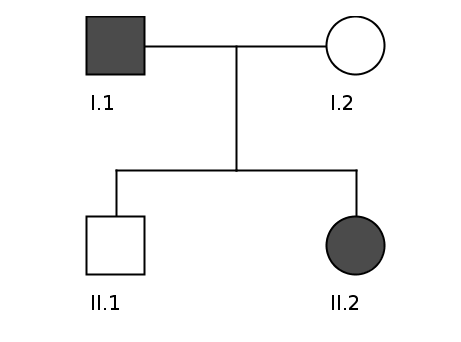
\includegraphics[width=.4\textwidth]{./img/ADpedigree.png}
\caption{An example pedigree representing a family segregating an autosomal dominantly inherited disease. The father I.1 is assumed to be a heterozygous mutation carrier, while the mother has the wildtype sequence. The daughter II.2 is affected and is a heterozygous mutation carrier, while the son II.1 is healthy and has the wildtype sequence. }
\label{fig:ad}
\end{figure}

For autosomal dominant inheritance, arbitrary family structures may be analyzed. Genes are filtered based on the occurrence of a variant that is heterozygous in all affected individuals and not present in the healthy individuals.

For the family shown in Figure~\ref{fig:ad}, we can write the PED file as follows:

\begin{Verbatim}[frame=single]
FAM2	I.1	 0	  0	  1	2
FAM2	I.2	 0	  0	  2	1
FAM2	II.1	I.1	I.2	1	1
FAM2	II.2	I.1	I.2	2	2
\end{Verbatim}

\end{homeworkSection}

\begin{homeworkSection}{X chromosomal recessive pedigrees}
A family segregating an X chromosomal recessive disease is shown in Figure~\ref{fig:xr}.
\begin{figure}[!ht]
 \centering
 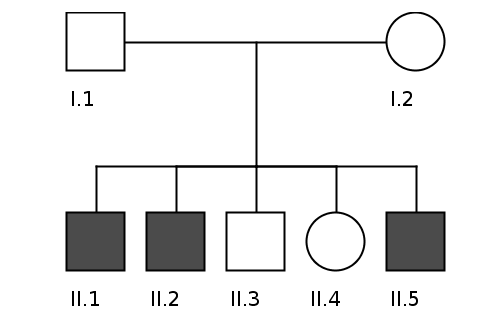
\includegraphics[width=.4\textwidth]{./img/XRpedigree.png}
\caption{An example pedigree representing a family segregating an X chromosomal recessive disease. The mother I.2 must be a heterozygous mutation carrier. Each of the affected sons is hemizygous for the mutation (this is generally called as homozygous ALT in VCF files). Unaffected sons must display the wildtype sequence, whereas daughters my be heterozygous for the mutation or may have the wildtype sequence.}
\label{fig:xr}
\end{figure}



For the family shown in Figure~\ref{fig:xr}, we can write the PED file as follows:

\begin{Verbatim}[frame=single]
FAM3	I.1	 0	  0	  1	1
FAM3	I.2	 0	  0	  2	1
FAM3	II.1	I.1	I.2	1	2
FAM3	II.2	I.1	I.2	1	2
FAM3	II.3	I.1	I.2	1	1
FAM3	II.4	I.1	I.2	2	1
FAM3	II.5	I.1	I.2	2	2
\end{Verbatim}
\end{homeworkSection}

\end{homeworkProblem}
%%%%%%%%%%%%%%%%%%%%%%%%%%%%%%%%%%%%%%%%%%%%%%%%%%%%%%%%%%%%%%%%%%%%%%%%%%%
%%%%%%%%%%%%%%%%%%%%%%%%%%%%%%%%%%%%%%%%%%%%%%%%%%%%%%%%%%%%%%%%%%%%%%%%%%%

\begin{homeworkProblem}[8. Integrating Pedigree Analysis with Annotation of VCF Files with Jannovar]
This example will present a complete tutorial for creating a program that will perform simple pedigree analysis based on the data in a multisample VCF file representing a family that is segregating a Mendelian disease together with the corresponding PED file. The goal of this kind of analysis is to filter the data in the VCF file for genes with variants that are compatible with the indicated mode of inheritance in the family.

There are many ways of building Java programs from source, and different users will most likely stick to their favorite tools. However, in order to present a complete and functional example using the Jannovar.jar file as a Java library, we will present a complete build system using apache ant\footnote{Apache Ant is a command-line tool that is used to build Java applications, similar to ``make'' for C programs. See http://ant.apache.org/.} to build the program.


The tutorial comes with a compressed directory called ``tutorialcode.tgz''. Download and uncompress this
\begin{verbatim}
$ tar xvfz tutorialcode.tgz
\end{verbatim}
The directory contains a subdirectory \texttt{src/jped} that contains the Java class (\texttt{JPed.java}) we will develop for this tutorial. Note that the directory contains another directory called lib. You will need to copy the latest version of \texttt{Jannovar.jar} into this directory (if you have a Jannovar version such as \texttt{jannovar-1.0.jar}, please rename the file to \texttt{Jannovar.jar}). Entering the following ant command will cause the executable to be built.
\begin{verbatim}
$ ant jped
\end{verbatim}


We can now run the code using the PED file fam1.ped and the VCF file sample.vcf. This contains one gene with a homozygous mutation compatible with autosomal recessive inheritance.

\begin{verbatim}
$ java -jar JPed.jar -D ucsc_hg19.ser -V sample.vcf -P fam1.ped -I AR
\end{verbatim}            

The program will then print its results to a file called \texttt{jped.txt}.:

\begin{scriptsize}
\begin{verbatim}
The following genes have variants that are compatible with autosomal recessive inheritance
CDHR2
MISSENSE	CDHR2	CDHR2(uc021yie.1:exon13:c.1271T>C:p.V424A)	chr5:g.176004476T>C	0/0:0/1:0/1:0/0:0/1
MISSENSE	CDHR2	CDHR2(uc021yie.1:exon14:c.1393A>C:p.M465L)	chr5:g.176004680A>C	0/1:0/0:0/1:0/1:0/1
GML
MISSENSE	GML	GML(uc003yxg.3:exon3:c.160C>T:p.R54C)	chr8:g.143922620C>T	0/1:0/1:1/1:0/1:1/1
\end{verbatim}
\end{scriptsize}

That is, there is a compound heterozygous mutation in \textit{CDHR2} and a homozygous mutation in \textit{GML}.



\begin{homeworkSection}{Understanding the Java code of JPed}
JPed is a java program that uses the Jannovar to perform pedigree analysis and variant annotation. It is not by any means a complete program, but rather intends to demonstrate how to use the Jannovar library as a component of more sophisticated Exome analysis pipelines. The following sections explain the code  to show the functionality of the Jannovar library. Further help for programming with Jannovar can be obtained from the Javadoc documentation that comes with this distribution.
\end{homeworkSection}

\begin{homeworkSection}{Imports}
 Most Java programs import various programming libraries to perform various tasks. This is done after the package declaration and before the actual class definition. JPed first imports some standard Java libraries and then imports various classes from Jannovar to perform annotation, genotype calling, and pedigree analysis. Most programs using Jannovar will get by with these import declarations, but some additional functionality is available from other classes (consult the Javadoc API).


\begin{lstlisting}
package jped;

import java.io.BufferedWriter;
import java.io.FileWriter;
import java.io.IOException;
import java.util.ArrayList;
import java.util.HashMap;
import java.util.Iterator;
import java.util.Map;
import java.util.Collections;

/** Command line parser from apache */
import org.apache.commons.cli.CommandLine;
import org.apache.commons.cli.GnuParser;
import org.apache.commons.cli.HelpFormatter;
import org.apache.commons.cli.Option;
import org.apache.commons.cli.Options;
import org.apache.commons.cli.ParseException;
import org.apache.commons.cli.Parser;

/** Classes from the Jannovar library. */
import jannovar.annotation.Annotation;
import jannovar.annotation.AnnotationList;
import jannovar.common.VariantType;
import jannovar.exception.JannovarException;
import jannovar.exome.Variant;
import jannovar.genotype.GenotypeCall;
import jannovar.io.PedFileParser;
import jannovar.io.SerializationManager;
import jannovar.io.VCFReader;
import jannovar.pedigree.Pedigree;
import jannovar.reference.Chromosome;
import jannovar.reference.TranscriptModel;
\end{lstlisting}

\end{homeworkSection}

\begin{homeworkSection}{Class declaration and class-level variables}
 Following the declaration of the class JPed, we declare the following variables:
\begin{center}
\begin{tabular}{ll}
chromosomeMap & Will contain the genomic transcript data for the annotations\\
variantList & Will contain the list of variant found in the VCF file\\
sampleNames & Will contain the sample names found in the VCF file \\
pedigree & Will contain an object representing the pedigree in the PED file\\
geneMap &  Genes encountered during parsing of VCF file. \\
\end{tabular}
\end{center}


\begin{lstlisting}
public class JPed {

    private HashMap<Byte,Chromosome> chromosomeMap=null;
    private ArrayList<Variant> variantList=null;
    private ArrayList<String> sampleNames = null;
    private Pedigree pedigree = null;
    private HashMap<String,Gene> geneMap=null;
\end{lstlisting}

\end{homeworkSection}

\begin{homeworkSection}{Gene: A simple class}
 Many types of analysis in human genetics occur on the gene level. For instance, we look if a gene has two distinct heterozygous variants with maternal and paternal inheritance in order to identify a candidate compound heterozygous mutation in an autosomal recessive disorder. In realistic applications, one might want to have a \texttt{Gene} class with many sophisticated analysis functions, but for JPed, we will define a minimal \texttt{Gene} class that basically holds the gene symbol, as well as lists of the Variants and the corresponding annotations. Note that \texttt{Variant} is a Jannovar class that represents a single variant identified in a VCF file, and stores information such as the chromosomal location, the quality of the variant call, and the genotype. The annotations in the simple \texttt{Gene} class are stored as Strings. The \texttt{Gene} class is defined as an inner class of JPed.

\begin{lstlisting}
 public class Gene {
	public String symbol;
	public ArrayList<String> annots;
	public ArrayList<Variant> vars;
	public Gene (String s) {
	    this.symbol = s;
	    this.vars = new ArrayList<Variant>();
	    this.annots = new ArrayList<String>();
	}
	public void addVariant(Variant v, String a) {
	    this.vars.add(v);
	    this.annots.add(a);
	}
	public void print() {
	  System.out.println(symbol);
	  for (String a : annots) {
	    System.out.println(a);
	  }
	}
    }
\end{lstlisting}


\end{homeworkSection}
\begin{homeworkSection}{The constructor}
 The constructor of the JPed class initializes the HashMap \texttt{geneMap}, which will store all of the genes that we encounter during parsing of the VCF file.


\begin{lstlisting}
public JPed() {
	this.geneMap = new HashMap<String,Gene>();
   } 
\end{lstlisting}

\end{homeworkSection}

\begin{homeworkSection}{The main function}
The main function first parses the arguments from the command line:
\begin{enumerate}
 \item The serialize transcript data file (e.g., \verb+ucsc_hg19.ser+)
\item A VCF file
\item A corresponding PED file
\item A mode of inheritance (must be one of AD (autosomal dominant), AR (autosomal recessive) or X (X chromosomal)
\end{enumerate}
 JPed use the command line library CLI from the Apache foundation to parse the arguments.\footnote{See
http://commons.apache.org/proper/commons-cli/ for details.}

After this, the program performs the following tasks
\begin{enumerate}
 \item Construction of a JPed object
\item Deserialization (``decompression'') of the serialized transcript data file 
\item Annotation of the VCF file (creation of a list of Variants) 
\item Processing of the variants to get an annotation string for each variant and to add variants to a gene object depending on their gene symbol
\item Parsing (input) of the PED filename
\item Filtering of the genes by inheritance pattern. By default, all genes are tested for autosomal recessive, autosomal dominant, and X chromosomal recessive inheritance.
\end{enumerate}
Note that many of the functions in Jannovar throw exceptions if the input data is malformed or otherwise erroneous. If JPed catches any exception, it prints an error message and quits, but realistic programs would probably implement more sophisticated error handling.

\begin{lstlisting}
public static void main(String argv[]) {
	try {
	    String transcriptModel = argv[0];
	    String vcfFile = argv[1];
	    String pedFile = argv[2];
	    JPed jped = new JPed();
	    jped.deserializeUCSCdata(transcriptModel);
	    jped.annotateVCF(vcfFile);
	    jped.processVariants();
	    jped.parsePedFile(pedFile);
	    jped.filterByInheritance();
	    
	} catch (Exception e) {
	    e.printStackTrace();
	    usage();
	    System.exit(1);
	}
    }
\end{lstlisting}

\end{homeworkSection}
\begin{homeworkSection}{Deserialization of Transcript Data}
The main Jannovar program can be used as explained above to create a transcript data file (for instance, \verb+ucsc_hg19.ser+). This file can then be used by Jannovar or other programs to extract data about transcripts that is needed for annotation. Jannovar provides a class \texttt{SerializationManager} that is used to deserialize (``decompress'') the file and create a list of \texttt{TranscriptModel} objects (there is one such object for each isoform). Jannovar also provides a class called \texttt{Chromosome} that can be used to create a HashMap of \texttt{Chromosome} objects from the \texttt{TranscriptModel} list. Internally, the \texttt{Chromosome} objects store the \texttt{TranscriptModel} objects as an interval tree, which allows for quick and reliable searches.
 


\begin{lstlisting}
public void deserializeUCSCdata(String path) throws JannovarException {
	SerializationManager manager = new SerializationManager();
	ArrayList<TranscriptModel> kgList = manager.deserializeKnownGeneList(path);
	this.chromosomeMap = Chromosome.constructChromosomeMapWithIntervalTree(kgList);
}  
\end{lstlisting}

\end{homeworkSection}

\begin{homeworkSection}{Input VCF Data}
Jannovar provides the class \texttt{VCFReader}, which is used to input VCF data and extract a list of \texttt{Variant} objects (in the class variable \texttt{variantList}) as well as a list of the names of the samples represented in the VCF file (in the class variable \texttt{sampleNames}).

\begin{lstlisting}
public void annotateVCF(String path) throws JannovarException {
	VCFReader parser = new VCFReader();
	parser.parseFile(path);
	this.variantList = parser.getVariantList();
	this.sampleNames = parser.getSampleNames();
 }
\end{lstlisting}
\end{homeworkSection}


\begin{homeworkSection}{Grouping variants to genes}
In this example, we group the variants to Genes (see the \texttt{Gene} class above). Thus, we will group the \texttt{Variant}s to the genes they belong to. This is a very simple function, but
more sophisticated exome analysis pipelines would probably want to filter the variants at this point in the analysis. For instance, the code could compare the variants to databases of common variants form dbSNP or in-house databases. Instead, the code groups the variants according to the gene symbol (alternatively, the function \texttt{getGeneId()} is provided, which will return the Entrez Gene ID for ucsc.ser or the ENSEMBL Gene ID for ensembl.ser). The function also retrieves a String representing the main annotation for the variant using the function \texttt{annotateVariant} (see below).

\begin{lstlisting}
public void processVariants() throws JannovarException {
	for (Variant v: this.variantList) {
	    String sym = v.getGeneSymbol();
	    String annot = annotateVariant(v);
	    Gene g = null;
	    if (this.geneMap.containsKey(sym)) {
		  g = this.geneMap.get(sym);
	    } else {
		 g = new Gene(sym);
		 this.geneMap.put(sym,g);
	     }
	     g.addVariant(v,annot);
	}
    }
\end{lstlisting}


\end{homeworkSection}

\begin{homeworkSection}{Annotating variants}
This function extracts the chromosomal location, the reference and the alternate sequence, the genotype and the variant call quality from the Variant object. 

\begin{lstlisting}
private String annotateVariant(Variant v) throws JannovarException
    {
	byte chr =  v.getChromosomeAsByte();
	String chrStr = v.get_chromosome_as_string();
	int pos = v.get_position();
	String ref = v.get_ref();
	String alt = v.get_alt();
	String gtype = v.getGenotypeAsString();
	float qual = v.get_variant_quality();
    ....
\end{lstlisting}



It then passes this information to the \texttt{Chromosome} object representing the appropriate chromosome
 \begin{lstlisting}
  	Chromosome c = this.chromosomeMap.get(chr);
 \end{lstlisting}
Finally, it gets an \texttt{AnnotationList} object representing all of the annotations that match to the variant (one per affected isoform). It retrieves a single representative annotation (one with the highest priority class), and returns a string with all of the relevant information.
 \begin{lstlisting}
 	AnnotationList annL = c.getAnnotationList(pos,ref,alt);
	String annotation = annL.getSingleTranscriptAnnotation();
    	v.setAnnotation(annL);
	String effect = annL.getVariantType().toString();
	String sym = annL.getGeneSymbol();
	String s = String.format("%s\t%s\t%s\t%s\t%s",
		effect,sym,annotation,v.get_chromosomal_variant(),gtype);
	return s; 
}
 \end{lstlisting}

\end{homeworkSection}

\begin{homeworkSection}{Parsing the PED file}
Jannovar provides a class called \texttt{PedFileParser} to parse a PED file, and it stores the information in a class called 
\texttt{Pedigree}. The latter class is also used to perform pedigree analysis as described above.
 
\begin{lstlisting}
public void parsePedFile(String path) throws JannovarException {
	PedFileParser parser = new PedFileParser();
	this.pedigree = parser.parseFile(path);
	this.pedigree.adjustSampleOrderInPedFile(this.sampleNames);
}
\end{lstlisting}
\end{homeworkSection}

\begin{homeworkSection}{Simple pedigree analysis}
 
To demonstrate the pedigree filtering capabilities of Jannovar, we show a function that performs filtering of the genes in the VCF file according to whether they are inherited in an autosomal recessive, autosomal dominant, or X chromosomal recessive fashion. In a sophisticated analysis pipeline, one would probably want to filter out all variants that are unlikely to be pathogenic before this step (e.g., INTRONIC variants). But then, the actually filtering is easy.
The function basically passes a list of \texttt{Variant} objects corresponding to a given gene to the pedigree functions

\begin{itemize}
 \item isCompatibleWithAutosomalRecessive (also: homozygous and compound het variants)
 \item isCompatibleWithAutosomalRecessiveHomozygous (only homozygous variants are considered)
 \item isCompatibleWithAutosomalRecessiveCompoundHet (only compound heterozygous variants are considered)
\item isCompatibleWithAutosomalDominant
\item isCompatibleWithXChromosomalRecessive
\end{itemize}

In this function, all of the variants corresponding to a gene are passed to the pedigree object for analysis, but other analysis pipelines could be implemented and would need only to deliver a list of \texttt{Variant} objects chosen according to some criterion. The function \verb+filterByInheritance()+ prints out whether any of the genes in the VCF file are compatible with the indicated mode of inheritance. Additionally standard Java code for writing to a file is not shown here.

\begin{lstlisting}
 for (Gene g : this.geneMap.values()) {
		ArrayList<Variant> varList = g.vars;
		if (this.mode==inheritanceMode.AR && 
		    this.pedigree.isCompatibleWithAutosomalRecessive(varList)) {
		    out.write(g.getAnnotations());
		} 
		else if (this.mode==inheritanceMode.HOM && 
		    this.pedigree.isCompatibleWithAutosomalRecessiveHomozygous(varList)) {
		    out.write(g.getAnnotations());
		} 
		else if (this.mode==inheritanceMode.COMPHET && 
		    this.pedigree.isCompatibleWithAutosomalRecessiveCompoundHet(varList)) {
		    out.write(g.getAnnotations());
		} 
		else if (this.mode==inheritanceMode.AD &&
		    this.pedigree.isCompatibleWithAutosomalDominant(varList)) {
		    out.write(g.getAnnotations());
		} 
		else if (this.mode==inheritanceMode.X &&
		    this.pedigree.isCompatibleWithXChromosomalRecessive(varList)) {
		     out.write(g.getAnnotations());
		} 
	    }
\end{lstlisting}
\end{homeworkSection}

\end{homeworkProblem}
%%%%%%%%%%%%%%%%%%%%%%%%%%%%%%%%%%%%%%%%%%%%%%%%%%%%%%%%%%%%%%%%%%%%%%%%%%%
%%%%%%%%%%%%%%%%%%%%%%%%%%%%%%%%%%%%%%%%%%%%%%%%%%%%%%%%%%%%%%%%%%%%%%%%%%%
\begin{homeworkProblem}[9. Running JPed]
We can now run the JPed program to illustrate its usage. You will find a VCF file called sample.vcf in the tutorial directory. This file has variants that correspond to five different genes, and there are genotypes for the five persons
I.1 (the father), I.2 (the mother), II.1 (first son), II.2 (second son), and II.3 (daughter). We have provided three different PED files corresponding to autosomal recessive, autosomal dominant, and X chromosomal recessive inheritance. One of the genes in the VCF file sample.vcf is compatible with each of the inheritance modes, as explained in the following text.

\begin{homeworkSection}{Autosomal Recessive Inheritance}
 We start off with the pedigree and the PED file from above (Shown here again for convenience as Figure~\ref{fig:ar2}).

\begin{figure}[!ht]
 \centering
 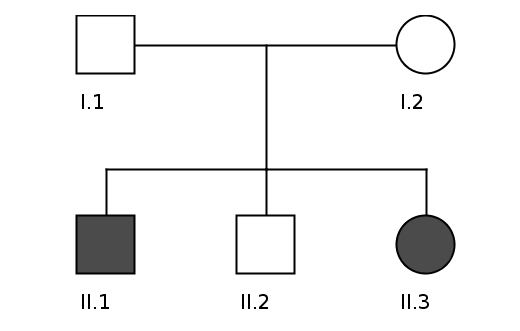
\includegraphics[width=.4\textwidth]{./img/ARpedigree.png}
\caption{An example pedigree representing a family segregating an autosomal recessively inherited disease.}
\label{fig:ar2}
\end{figure}


The PED file.

\begin{Verbatim}[frame=single]
FAM1	I.1	 0	  0	  1	1
FAM1	I.2	 0	  0	  2	1
FAM1	II.1	I.1	I.2	1	2
FAM1	II.2	I.1	I.2	1	1
FAM1	II.3	I.1	I.2	2	2
\end{Verbatim}

JPed produces the output for the following gene (See Table~\ref{tab:CDHR2}):

\begin{scriptsize}
\begin{verbatim}
[JPed] Compatible with autosomal recessive: CDHR2
MISSENSE	CDHR2	CDHR2(uc021yie.1:exon13:c.1271T>C:p.V424A)	chr5	176004476	T	C	0/0:0/1:0/1:0/0:0/1193.0
MISSENSE	CDHR2	CDHR2(uc021yie.1:exon14:c.1393A>C:p.M465L)	chr5	176004680	A	C	0/1:0/0:0/1:0/1:0/1782.0
\end{verbatim}
\end{scriptsize}


\begin{table}[!ht]
\begin{center}
\begin{tabular}{llllll}
\toprule
Variant  & Father (I.1) & Mother (I.2) & Son 1 (II.1) & Son 2 (II.2) & Daughter (II.3)\\
\midrule
V424A & ref & het & het & ref & het\\
M465L & het & ref & het & het & het\\
\bottomrule
\end{tabular}
\end{center}
\caption{The \textit{CDHR2} is compatible with autosomal recessive inheritance. The VCF file has two variants in a gene that are compatible with autosomal recessive because they are compound heterozygous in both affected children, and the unaffected child is heterozygous for only one of the variants. Each parent is heterozygous for a different variant.}
\label{tab:CDHR2}
\end{table}

On the other hand, there are two variants that corresponding to the WWC1 gene. 

\begin{scriptsize}
\begin{verbatim}
5	176004476	.	T	C	193.23	PASS	QD=11.71;	GT:GQ	0/0:99	0/1:99	0/1:99	0/1:99	0/1:99
5	176004680	.	A	C	781.93	PASS	QD=11.71;	GT:GQ	0/1:99	0/0:99	0/1:99	0/1:99	0/1:99 
\end{verbatim}
\end{scriptsize}

In this case, the gene is not compatible with autosomal recessive inheritance, because both variants come from the father: the father is thus himself carrier of two variants but is healthy; therefore, the variants cannot be the cause of an autosomal recessive disease (Table~\ref{tab:WWC1}).

\begin{table} [!ht]
\begin{center}
\begin{tabular}{llllll}
\toprule
Variant  & Father (I.1) & Mother (I.2) & Son 1 (II.1) & Son 2 (II.2) & Daughter (II.3)\\
\midrule
p.R49C & het & ref & het & ref & het\\
p.133\_134del & het & ref & het & het & het\\
\bottomrule
\end{tabular}
\end{center}
\caption{The WWC1 gene is not compatible with autosomal recessive inheritance, because both variants come from the father}
\label{tab:WWC1}
\end{table}



Similarly, the HK3 has two variants that are found not to be compatible with autosomal recessive inheritance because the unaffected child is compound heterozygous (Table



\begin{table} [!ht]
\begin{center}
\begin{tabular}{llllll}
\toprule
Variant  & Father (I.1) & Mother (I.2) & Son 1 (II.1) & Son 2 (II.2) & Daughter (II.3)\\
\midrule
p.Q156H & het & ref & het & het & het\\
p.Q134R & het & ref & het & het & het\\
\bottomrule
\end{tabular}
\end{center}
\caption{The HK3 gene is not compatible with autosomal recessive inheritance, because the unaffected child is compound heterozygous.}
\label{tab:HK3}
\end{table}


The FGFR4 gene is not compatible with autosomal recessive inheritance, because one of the affected children only has one of the two heterozygous variants.

\begin{table} [!ht]
\begin{center}
\begin{tabular}{llllll}
\toprule
Variant  & Father (I.1) & Mother (I.2) & Son 1 (II.1) & Son 2 (II.2) & Daughter (II.3)\\
\midrule
p.P136L & het & ref & het & ref & het\\
p.G388R & het & ref & het & het & het\\
\bottomrule
\end{tabular}
\end{center}
\caption{The FGFR4 gene is not compatible with autosomal recessive inheritance, because the unaffected child is compound heterozygous (p.P136L,p.G388R).}
\label{tab:FGFR4}
\end{table}


Finally, the GML gene is compatible with autosomal recessive inheritance based on a homozygous variant.

\begin{table} [!ht]
\begin{center}
\begin{tabular}{llllll}
\toprule
Variant  & Father (I.1) & Mother (I.2) & Son 1 (II.1) & Son 2 (II.2) & Daughter (II.3)\\
\midrule
p.R54C & het & het & hom & het & hom\\
\bottomrule
\end{tabular}
\end{center}
\caption{The GML gene is  compatible with autosomal recessive inheritance, because the affected children are homozygous, both parents are heterozygous, and the unaffected child is heterozygous.}
\label{tab:GML}
\end{table}


\end{homeworkSection}



 
\begin{homeworkSection}{Autosomal dominant}
Let us now investigate the same data using a different PED file representing autosomal dominant inheritance (Fig.~\ref{fig:ad2})



\begin{figure}[!ht]
 \centering
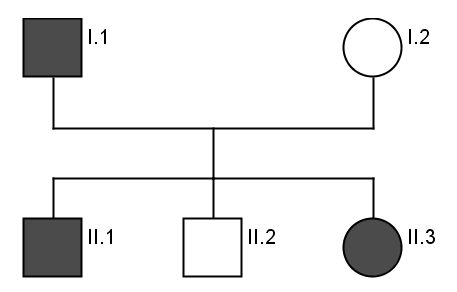
\includegraphics[width=.4\textwidth]{./img/ADped2.png}
\caption{An  pedigree representing a family segregating an autosomal dominant inherited disease.}
\label{fig:ad2}
\end{figure}


The PED file (available as \texttt{fam2.ped} in the tutorial directory).

\begin{Verbatim}[frame=single]
FAM1	I.1	 0	  0	  1	2
FAM1	I.2	 0	  0	  2	1
FAM1	II.1	I.1	I.2	1	2
FAM1	II.2	I.1	I.2	1	1
FAM1	II.3	I.1	I.2	2	2
\end{Verbatim}

We perform the analysis as follows:


\begin{verbatim}
$ java -jar JPed.jar -D ucsc_hg19.ser -V sample.vcf -P fam2.ped -I AD
\end{verbatim}   

This writes the following results to the file \texttt{jped.txt}. Note that all of the variants in 
each gene that has at least one variant compatible with autosomal dominant inheritance is written to the
file. The first line of the file indicates the mode of inheritance being sought, and the second line
shows a summary of the pedigree that helps to quickly interpret the results (recall that 0/0 is homozygous reference,
0/1 is heterozygous, and 1/1 is homozygous alternate).
\begin{scriptsize}
 \begin{verbatim}
The following genes have variants that are compatible with autosomal dominant inheritance
FAM1:I.1[affected;father]:I.2[unaffected;mother]:II.1[affected;male]:II.2[unaffected;male]:II.3[affected;female]
FGFR4
MISSENSE        FGFR4   FGFR4(uc003mfl.3:exon4:c.407C>T:p.P136L)        chr5:g.176517797C>T     0/1:0/0:0/1:0/0:0/1
MISSENSE        FGFR4   FGFR4(uc003mfl.3:exon9:c.1162G>A:p.G388R)       chr5:g.176520243G>A     0/0:0/1:0/1:0/0:0/0
WWC1
MISSENSE        WWC1    WWC1(uc003lzw.3:exon2:c.145C>T:p.R49C)  chr5:g.167835539C>T     0/1:0/0:0/1:0/0:0/1
NON_FS_DELETION WWC1    WWC1(uc010jjf.1:exon4:c.399_401del:p.133_134del)        chr5:g.167881030GGA>-   0/1:0/0:0/1:0/1:0/1
\end{verbatim}
\end{scriptsize}



The FGFR4 and the WWC1 genes are identified as candidates because they each have a single variant that is heterozygous in all affected persons (p.P136L in the case of FGFR4, and p.R49C in the case of WWC1).  There is another variant in the ZC3H3 gene (p.F149Y) that is not identified as compatible with autosomal dominant (Table~\ref{tab:ZC3H3}).

\begin{table} [!ht]
\begin{center}
\begin{tabular}{llllll}
\toprule
Variant  & Father (I.1) & Mother (I.2) & Son 1 (II.1) & Son 2 (II.2) & Daughter (II.3)\\
\midrule
p.F149Y & het & ref & het & het & het\\
\bottomrule
\end{tabular}
\end{center}
\caption{The ZC3H3 gene is not compatible with autosomal dominant inheritance. Even though all affected persons are heterozygous for the variant p.F149Y, the unaffected child II.2 is also heterozygous.}
\label{tab:ZC3H3}
\end{table}

\end{homeworkSection}


\begin{homeworkSection}{X Chromosomal Recessive}
Let us now investigate the same data using a different PED file representing X chromosomal recessive inheritance (Fig.~\ref{fig:xr2}).



\begin{figure}[!ht]
 \centering
 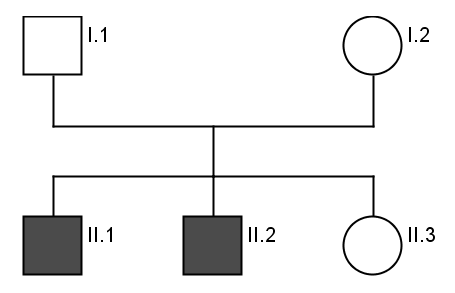
\includegraphics[width=.4\textwidth]{./img/XRped2.png}
\caption{An  pedigree representing a family segregating an X chromosomal recessive  disease.}
\label{fig:xr2}
\end{figure}


The PED file (available as \texttt{fam3.ped} in the tutorial directory).

\begin{Verbatim}[frame=single]
FAM1	I.1	 0	  0	  1	1
FAM1	I.2	 0	  0	  2	1
FAM1	II.1	I.1	I.2	1	2
FAM1	II.2	I.1	I.2	1	2
FAM1	II.3	I.1	I.2	2	1
\end{Verbatim}

We perform the analysis as follows:

\begin{verbatim}
$ java -jar JPed.jar -D ucsc_hg19.ser -V sample.vcf -P fam3.ped -I X
\end{verbatim}   

None of the above variants are identified as compatible with X chromosomal inheritance, simply because the genes are not located on the X chromosome. The following variant is identified as compatible with X chromosomal inheritance (Table~\ref{tab:TCEANC}).



\begin{table} [!ht]
\begin{center}
\begin{tabular}{llllll}
\toprule
Variant  & Father (I.1) & Mother (I.2) & Son 1 (II.1) & Son 2 (II.2) & Daughter (II.3)\\
\midrule
p.W351L & ref & het & hom & hom & ref\\
\bottomrule
\end{tabular}
\end{center}
\caption{The TCEANC gene is  compatible with X chromosomal inheritance. The mother is heterozygous and all affected sons are called as homozygous (actually, they are hemizygous).}
\label{tab:TCEANC}
\end{table}


Finally, a variant in the MAGEB3 gene (p.I112T; chrX:g.30254376T$>$C) is correctly not called as compatible with X chromosomal inheritance because the son II.2 has the reference sequence, and another variant in the FAM47A gene (p.E507Q; chrX:g.34148877C$>$G) is correctly not called as compatible with X chromosomal inheritance because the both the father and the mother are heterozygous for the variant and the healthy daughter is homozygous for it.

\end{homeworkSection}
\cite{Zhang2003}
\end{homeworkProblem}



%%%%%%%%%%%%%%%%%%%%%%%%%%%%%%%%%%%%%%%%%%%%%%%%%%%%%%%%%%%%%%%%%%%%%%%%%%%
%%%%%%%%%%%%%%%%%%%%%%%%%%%%%%%%%%%%%%%%%%%%%%%%%%%%%%%%%%%%%%%%%%%%%%%%%%%
\begin{homeworkProblem}[10. Three additional applications built with the Jannovar library]
We provide two additional examples of how to use Jannovar as a programming library. We will not provide any explanation of the code in this tutorial since the Java code itself is documented. Instead, we will merely provide an introduction on how to uses the example programs, which are again not intended to be full fledged applications for use in exome pipelines, but rather intend to demonstrate how to use Jannovar in your own applications.

\begin{homeworkSection}{JLink}
Filtering a VCF file for variants in a linkage interval
If a linkage interval is available to filter the results of exome sequencing, one may start the analysis of exome data by looking for potentially pathogenic variants located in the linkage interval.
To build the application enter
\begin{verbatim}
$ ant jlink
\end{verbatim}
The application is run with the following command
\begin{verbatim}
$ java -jar JLink.jar -V vcffile -D jfile -I interval [-O ofile]
\end{verbatim}
The interval is indicated as ``chr:start-end''. For instance, to indicate an interval from 1 to 2 million on chromosome 7, use \verb+chr7:1000000-2000000+. If you indicate an outfile with the \verb+-O+ flag, results will be written to file (all variants of pathogenicity class 1 that are located in the linkage interval, see Table~~\ref{tab:priority} for the priority class of the different categories of variant).

\end{homeworkSection}

\begin{homeworkSection}{JQCVCF}
There are some quality measures that are useful for exome analysis. The application JQCVCF provides a start of an application that might be useful for this purpose. To build the application, enter:
\begin{verbatim}
$ ant jqc
\end{verbatim}
To run the application, enter
\begin{verbatim}
$ java -jar JQCVCF.jar -D ucsc_hg19.ser -V filename.vcf 
\end{verbatim}
This will automatically create a latex file called \texttt{jqc.tex}. 

The code basically generates a report on the following parameters.

\paragraph{Ti/Tv (sometimes called Ts/Tv)}:

The transition/transversion (Ti/Tv) ratio  has been used by
multiple studies as a quality control parameter for
checking the overall SNP quality. 

The Ti/Tv ratio is computed as the
number of transition SNPs divided by the number of transversion
SNPs. Different specific genetic regions will display different Ti/Tv ratios.
Note that there are twice as many possible transversions as transitions, and therefore, if there were no biological bias one might expect Ti/Tv=0.5. However, the actual Ti/Tv ratio differs by genomic regions. For
human genome data, the Ti/Tv ratio is around 3.0 for SNPs inside exons
and about 2.0 elsewhere, and the ratio also differs between
synonymous and non-synonymous SNPs. Because the target regions of
exome capture kits often cover more than just exons, the Ti/Tv ratio
for SNPs inside these target regions is expected to lie between 2.0
and 3.0 with the value depending on the fraction of exons inside
target regions.   Another possible reason for the greater transition content of the exome is 
because the exome is under stronger selective pressure against missense mutations, whereas many transitions are tolerated as silent mutations because transitions in the third base of a codon rarely change the amino acid.



\paragraph{ns/ss}:
This is the ratio of non-synonymous substitutions (per site) to synonymous substitutions (per site). 
Since synonymous substitutions are better tolerated by evolution,  the ratio is expected to be below 1 
 but random errors would skew it upward. There are no accepted normal values, but we have generally seen values between 0.8 and 1.0.
 \paragraph{het/hom}: het/hom is the ratio of heterozygous to homozygous variant genotypes across all sample-site combinations. There are no accepted normal values, but populations with recent admixture will skew towards heterozygosity, whereas populations with inbreeding will skew towards homozygosity. We have generally seen values between 1.3 and 2.0.

\paragraph{Example}:
The following tables were generated by using JQVCF on the VCF file presented in Glusman G et al. (2012) Low budget analysis of Direct-To-Consumer genomic testing familial data. {\it F1000Research}.  {\bf 1}:3.

\begin{center}
\begin{tabular}{p{5cm}p{5cm}p{3cm}}
\hline
Parameter & Value & Range\\ 
\hline
Variant call Phred score & $88.8\pm 99.0$; median: 23.2 & [$\ >30$]\\ 
Total variants called & 37299 & [$>25,000$]\\ 
Transitions & 24205& - \\ 
Transversions & 11468& - \\ 
Ti/Tv  & 2.111 & [2-3]  \\ 
Synonymous &  4617 & -  \\ 
Nonsynonymous &  5355& - \\ 
ns/ss & 1.160 & [0.8-1.0] \\ 
Het calls & 33937& - \\ 
Hom calls & 1736& - \\ 
Het/Hom & 19.549& [1.3-2.0] \\ 
\hline
\end{tabular}
\end{center}


\vspace{1cm}

\begin{center}
\begin{tabular}{p{6cm}p{4cm}}
\hline
\multicolumn{2}{l}{Variant Distribution}\\ 
\hline 
Variant type & Count\\ 
\hline
missense & 5355\\ 
stopgain & 61\\ 
frameshift deletion & 69\\ 
frameshift insertion & 83\\ 
frameshift substitution & 4\\ 
nonframeshift deletion & 97\\ 
nonframeshift insertion & 79\\ 
splicing & 63\\ 
stoploss & 11\\ 
noncoding RNA exonic & 1848\\ 
noncoding RNA splicing & 10\\ 
UTR3 & 1267\\ 
UTR5 & 874\\ 
synonymous & 4617\\ 
intronic & 18357\\ 
noncoding RNA intronic & 623\\ 
upstream & 246\\ 
downstream & 158\\ 
intergenic & 3469\\ 
\hline
\end{tabular}
\end{center}


\paragraph{PDF generation}
If JQCVCF is called with the \verb+--pdf+ flag, it will attempt to compile the latex file using pdflatex, which should be
installed by default on most Linux systems. This will produce  a file called \texttt{jqc.pdf}. This option will not work without some modifications on most Windows and Mac systems, but users can compile the latex file separately (e.g., with MiKTeX on Windows systems). 

\paragraph{Distance threshold}
In some cases it may be desirable to restrict the Q/C analysis to variants that are on target or very near to it, since off target variant calls tend to be lower quality than on target calls. This can be done with the \verb+--threshold+ flag. For instance, the following call with restrict Q/C analysis to calls with 10 nucleotides of the target (any annotated exon) and output a PDF file:

\begin{small}
\begin{verbatim}
$ java -Xmx1g -jar JQCVCF.jar -D ucsc_hg19.ser -V mysample.vcf  --threshold 10 --pdf
\end{verbatim}
\end{small}




\end{homeworkSection}


\begin{homeworkSection}{JGeneCount}
Finally, there is an application that will print out the names of all the genes located in a 
given chromosomal interval For instance, the command
\begin{verbatim}
$ java -jar JGeneCount.jar -D ucsc_hg19.ser -I chr14:29781404-30552936 
\end{verbatim}
 will yield:
\begin{Verbatim}[frame=single]
Genes and transcripts in 14:29781404-30552936
1) MIR548AI
2) PRKD1
3) BC062469
4) U6
4 genes with 1 coding and 4 noncoding transcripts
\end{Verbatim}

This kind of information may be useful when evaluating copy number variants, for instance.
 
\end{homeworkSection}


 
\end{homeworkProblem}



%%%%%%%%%%%%%%%%%%%%%%%%%%%%%%%%%%%%%%%%%%%%%%%%%%%%%%%%%%%%%%%%%%%%%%%%%%%
%%%%%%%%%%%%%%%%%%%%%%%%%%%%%%%%%%%%%%%%%%%%%%%%%%%%%%%%%%%%%%%%%%%%%%%%%%%
\begin{homeworkProblem}[11. Documentation]
To create Javadoc documentation for Jannovar, download the maven repository from GitHub as described above and enter
\begin{verbatim}
$ mvn javadoc:javadoc
\end{verbatim}
This will create a directory called \verb+site/api-docs+ which will contain the Javadoc files.

 
\end{homeworkProblem}
%%%%%%%%%%%%%%%%%%%%%%%%%%%%%%%%%%%%%%%%%%%%%%%%%%%%%%%%%%%%%%%%%%%%%%%%%%%
%%%%%%%%%%%%%%%%%%%%%%%%%%%%%%%%%%%%%%%%%%%%%%%%%%%%%%%%%%%%%%%%%%%%%%%%%%%

\begin{homeworkProblem}[12. Troubleshooting]
\begin{homeworkSection}{Memory issues}
The java virtual machine reserves a certain amount of memory at the start of execution and cannot increase the amount of heap space if it runs out during execution. For this reason, users may need to ``reserve'' sufficient memory using the -Xmx and -Xmx flags. For instance, more memory is needed to annotate a VCF file representing a genome sequence than one representing an exome sequence. For instance, to reserve 8 gigabytes memory for Jannovar, enter the following:

\begin{verbatim}
$ java -Xms8G -Xmx8G -jar Jannovar.jar -D ucsc.ser sample.vcf
\end{verbatim}

Usually, 2 Gb should be more than enough for an exome or a genome annotation.

%\textcolor{red}{Jannovar does not need so much Memory annotating a VCF file if its iterating over the VCF. The more memory is used while processing the GFF files.}
\end{homeworkSection}

\begin{homeworkSection}{Network issues}
 If you use Jannovar to automatically download transcript data from the net and see an error message, check that the remote server is ``up'' and try again if necessary. If you are trying to download the data from behind a firewall, you may have to set the proxy using command line arguments (see above).
\end{homeworkSection}

\begin{homeworkSection}{Bugs}
 If you notice an annotation that is incorrect, please send a bug report to \texttt{marten.jaeger@charite.de} or \texttt{peter.robinson@charite.de}, including the VCF line that was incorrectly annotated, the output of Jannovar for that line, and the output as it should be. We have done our best to cover a very wide range of annotations, but as always in genetics, exceptions and oddities are common, and future versions of Jannovar will benefit from your input.
\end{homeworkSection}



\end{homeworkProblem}



%----------------------------------------------------------------------------------------

\end{document}
